\documentclass[12pt,a4paper]{article}
\usepackage{ctex}
\usepackage{graphicx}
\usepackage{geometry}
\usepackage{array}
\usepackage{setspace}
\usepackage{xeCJK}
\usepackage{indentfirst}
\usepackage{amsmath}
\usepackage{amsthm}
\usepackage{float}
\usepackage{subfigure}
\usepackage{booktabs}
\usepackage{multirow}
\usepackage{caption}
\usepackage{listings}
\usepackage{xcolor}
\usepackage{matlab-prettifier}
\usepackage{enumitem}
\captionsetup[table]{position=bottom}

% 页边距
\geometry{left=2.5cm,right=2.5cm,top=2.5cm,bottom=2.5cm}
% 默认宋体小四
\setCJKmainfont[BoldFont=SimHei]{SimSun}
\zihao{-4}
\linespread{1.25}

\lstdefinestyle{Matlab-boxed}{
  style=Matlab-editor,
  frame=single,
  framerule=0.6pt,
  rulecolor=\color{black},
  framesep=6pt,
  backgroundcolor=\color{black!2},
  basicstyle=\footnotesize\ttfamily,
}

\begin{document}
% 实验名称（小二黑体、居中）
\begin{center}
  {\zihao{2}\heiti 霍尔效应实验}
\end{center}
% 年级 专业 姓名 座位号（宋体小四、居中、段前后 0.5 行）
\vspace{0.1\baselineskip}
\begin{center}
  （\textbf{年级}\ \underline{2024 级}\quad \textbf{专业}\ \underline{x} \quad \textbf{姓名}\ \underline{Pinco Li} \quad \textbf{座位号} \ \underline{5}）
\end{center}
\vspace{0.1\baselineskip}

\section{实验目的}

\begin{enumerate}
  \item 了解霍尔效应及其副效应的产生原理及其消除方法
  \item 学习对称测量法在消除系统误差中的应用
  \item 测定励磁线圈的激励系数 $K_M(B)$ 和霍尔传感器的灵敏度 $K_H$
  \item 了解霍尔效应在现代科学技术中的应用，包括整数量子霍尔效应和分数量子霍尔效应
\end{enumerate}

\section{实验仪器}

\begin{figure}[H]
    \centering
    
\includegraphics[width=0.5\textwidth]{assets/实验装置1.jpg}
    \caption{霍尔效应实验装置($K_H=173.5 mV/(mA·T)$ \ $I_M=0.5A \ B=158mT$)}
    \label{fig:apparatus}
\end{figure}

\begin{enumerate}
    \item 霍尔效应实验仪主机（含励磁电流源、霍尔工作电流源、数字电压表）
    \item 霍尔效应实验附件（含励磁线圈、霍尔元件、磁场中可移动探测装置）
    \item 连接导线若干（两芯航空插座连接线、红黑香蕉插头连接线）
\end{enumerate}

\section{实验原理}

\subsection{霍尔效应的基本概念}

霍尔效应是1879年由美国物理学家霍尔（E. H. Hall）在研究导体载流子特性时发现的一种重要的物理现象。当一块有电流通过的金属或半导体薄板垂直地放在磁场中时，在垂直于电流和磁场的方向上，薄板的两个侧面之间会产生一个电势差，这种现象称为霍尔效应，所产生的电势差称为霍尔电压。

霍尔效应的产生机理可以这样理解：当导体中的载流子（电子或空穴）在电场作用下沿着导体运动时，若在垂直于电流的方向施加一个磁场，载流子在洛伦兹力的作用下会发生偏转。这种偏转使得载流子在导体的一侧积累，而在另一侧形成载流子的缺乏，从而在垂直于电流和磁场的方向上建立起一个横向电场，即霍尔电场。当霍尔电场产生的电场力与洛伦兹力平衡时，载流子的横向漂移停止，此时在导体两侧形成稳定的霍尔电压。

\subsection{霍尔电压与物理参数的关系}

对于厚度为 $d$、宽度为 $b$ 的半导体薄板，当工作电流 $I_S$ 沿着薄板流动，垂直于薄板表面的磁感应强度为 $B$ 时，薄板两侧产生的霍尔电压 $V_H$ 可以表示为：

\begin{equation}
V_H = R_H \frac{I_S B}{d} = K_H \cdot I_S \cdot B
\end{equation}

其中：
\begin{itemize}
    \item $R_H$ —— 霍尔系数，是材料的固有属性，单位为 m$^3$/C
    \item $K_H = R_H / d$ —— 霍尔元件的灵敏度，单位为 mV/(mA$\cdot$T) 或 mV/(mA$\cdot$kGs)
    \item $I_S$ —— 霍尔元件的工作电流，单位为 mA
    \item $B$ —— 垂直于半导体薄板的磁感应强度，单位为 T（特斯拉）或 Gs（高斯），其中 1T = 10$^4$ Gs
\end{itemize}

从上式可以看出，霍尔电压 $V_H$ 与工作电流 $I_S$ 和磁感应强度 $B$ 成正比。这一线性关系是霍尔元件作为磁场传感器和电流传感器的理论基础。

对于本实验使用的励磁线圈，其产生的磁感应强度 $B$ 与励磁电流 $I_M$ 存在如下关系：

\begin{equation}
B = K_M \cdot I_M
\end{equation}

其中 $K_M$ 称为励磁线圈的激励系数，单位为 T/A。将此式代入霍尔电压公式，可得：

\begin{equation}
V_H = K_H \cdot I_S \cdot K_M \cdot I_M
\end{equation}

\subsection{霍尔效应的副效应}

在实际测量中，霍尔电压的测量会受到多种副效应的影响，使测量结果产生系统误差。主要的副效应包括：

\textbf{1. 爱廷豪森效应（Ettingshausen Effect）}

当载流子在磁场中运动时，除了会发生横向偏转外，由于载流子的速度分布不均匀，快速运动的载流子和缓慢运动的载流子会分别向薄板的不同侧面聚集，导致两侧出现温度差。这种温度差会产生附加的温差电势 $V_E$，称为爱廷豪森效应。该效应产生的电压 $V_E$ 的极性与霍尔电压 $V_H$ 的极性相同，且 $V_E$ 随电流 $I_S$ 和磁场 $B$ 的方向同时改变而改变。

\textbf{2. 能斯特效应（Nernst Effect）}

由于霍尔元件工作电流引线焊点的不一致性，焊接点的接触电阻不同，通电后发热不均匀，引起温度分布不均。在磁场作用下，载流子会从高温区向低温区扩散，形成电压 $V_N$。能斯特效应产生的电压 $V_N$ 仅随磁场方向 $B$ 的改变而改变，与工作电流 $I_S$ 的方向无关。

\textbf{3. 里纪-勒杜克效应（Righi-Leduc Effect）}

这是一种由热扩散电流引起的二阶效应。当存在温度梯度时，热扩散会产生扩散电流。在磁场作用下，这些载流子也会受到洛伦兹力而发生偏转，产生类似于爱廷豪森效应的温差电势 $V_{RL}$。该电压 $V_{RL}$ 仅随磁场方向 $B$ 的改变而改变。

\textbf{4. 不等电势差（Unequal Potential Difference）}

由于霍尔元件材料的不均匀性以及焊接的不对称性，霍尔电压的引出电极不可能完全处在同一等势面上。因此，即使不加磁场，只要有工作电流 $I_S$ 流过，在电压输出端也会有一个不为零的电压 $V_0$。该电压 $V_0$ 随工作电流 $I_S$ 的方向改变而改变，但与磁场 $B$ 的方向无关。

\subsection{对称测量法消除副效应}

为了消除上述副效应对霍尔电压测量的影响，实验中采用对称测量法。具体方法是：分别测量工作电流 $I_S$ 和磁场 $B$ 的四种不同组合情况下的电压值，然后通过特定的数学组合来消除副效应的影响。

设 $I_S$ 正向为 $+I_S$，反向为 $-I_S$；磁场 $B$ 正向为 $+B$，反向为 $-B$。分别测量四种情况：

\begin{enumerate}
    \item 当 $I_S = +I_S$，$B = +B$ 时：
    \begin{equation}
    V_1 = V_H + V_0 + V_E + V_N + V_{RL}
    \end{equation}
    
    \item 当 $I_S = -I_S$，$B = +B$ 时：
    \begin{equation}
    V_2 = -V_H - V_0 - V_E + V_N + V_{RL}
    \end{equation}
    
    \item 当 $I_S = -I_S$，$B = -B$ 时：
    \begin{equation}
    V_3 = V_H - V_0 + V_E - V_N - V_{RL}
    \end{equation}
    
    \item 当 $I_S = +I_S$，$B = -B$ 时：
    \begin{equation}
    V_4 = -V_H + V_0 - V_E - V_N - V_{RL}
    \end{equation}
\end{enumerate}

对上述四个电压值进行如下运算：

\begin{equation}
\frac{1}{4}(V_1 - V_2 + V_3 - V_4) = V_H + V_E
\end{equation}

由于爱廷豪森效应产生的电压 $V_E$ 通常远小于霍尔电压 $V_H$（即 $V_E \ll V_H$），因此可以得到：

\begin{equation}
V_H \approx \frac{1}{4}(V_1 - V_2 + V_3 - V_4)
\end{equation}

在实际测量中，由于各电压值的符号已经通过实验装置的换向开关确定，我们通常取各次测量值的绝对值，然后计算平均值：

\begin{equation}
V_H \approx \frac{|V_1| + |V_2| + |V_3| + |V_4|}{4}
\end{equation}

这种对称测量法能够有效地消除不等电势差、能斯特效应和里纪-勒杜克效应的影响，大大提高了霍尔电压测量的准确性。

\subsection{霍尔效应的量子化现象}

在霍尔效应发现约100年后的1980年，德国物理学家克利青（Klaus von Klitzing）及其合作者 G. Dorda 和 M. Pepper 发现，在极低温度（液氦温度，约4.2 K）和强磁场（数十特斯拉）条件下，二维电子气系统的霍尔电阻呈现出量子化的台阶结构。这种现象被称为\textbf{整数量子霍尔效应}（Integer Quantum Hall Effect）。

整数量子霍尔效应中，霍尔电阻 $R_H$ 的量子化关系为：

\begin{equation}
R_H = \frac{V}{I} = \frac{h}{i e^2}, \quad i = 1, 2, 3, \ldots
\end{equation}

其中 $h$ 是普朗克常数，$e$ 是电子电荷，$i$ 是整数。这一发现不仅具有重要的基础物理意义，而且为精密测量提供了新的标准。从1990年起，国际上采用的电阻标准值为：

\begin{equation}
\frac{h}{e^2} = 25812.806 \text{ } \Omega
\end{equation}

其精度约为 $2 \times 10^{-8}$。克利青因这一重大发现获得了1985年诺贝尔物理学奖。

1982年，美国贝尔实验室的崔琦、斯托默（H. Stormer）和戈萨德（A. Gossard）在更低的温度和更强的磁场条件下，发现霍尔电阻在 $i = 1/3$、$1/5$、$2/5$ 等分数值处也出现了量子化的台阶，这种现象被称为\textbf{分数量子霍尔效应}（Fractional Quantum Hall Effect）。1983年，劳克林（R. Laughlin）从理论上成功解释了分数量子霍尔效应，提出了著名的劳克林波函数。这三位科学家因发现和解释分数量子霍尔效应而共同获得了1998年诺贝尔物理学奖。

近年来，中国科学家在量子霍尔效应研究领域也取得了重要突破。2010年，中国科学院物理研究所方忠、戴希团队与张首晟教授等合作，预言在磁性掺杂的拓扑绝缘体（如 Cr 或 Fe 掺杂的 Bi$_2$Te$_3$、Bi$_2$Se$_3$）中可以实现\textbf{量子反常霍尔效应}（Quantum Anomalous Hall Effect），这是一种无需外加磁场即可实现的量子霍尔效应。随后，清华大学薛其坤院士领导的团队在实验上成功观测到了这一效应，为未来低能耗电子器件的发展开辟了新的道路。

\section{实验步骤}

\subsection{实验连接与准备}

\begin{enumerate}
    \item 按照仪器面板上的文字和符号提示，将霍尔效应实验仪主机与霍尔效应实验附件架正确连接。\textbf{注意}：在连接前，必须将励磁电流 $I_M$ 和霍尔工作电流 $I_S$ 的调节旋钮逆时针旋至最小位置，确保初始电流为零。
    
    \item 使用两芯航空插座连接线，将主机面板上的励磁电流 $I_M$ 输出端与附件架上的 $I_M$ 励磁电流输入端连接。
    
    \item 使用红黑香蕉插头连接线，将主机面板上的 $I_S$ 霍尔工作电流输出端与附件架上的 $I_S$ 霍尔工作电流输入端连接。连接时必须注意极性：红色接线柱与红色接线柱对应相连，黑色接线柱与黑色接线柱对应相连。
    
    \item 使用红黑香蕉插头连接线，将主机面板上的 $V_H$ 霍尔电压测量端与附件架上的 $V_H$ 霍尔电压输出端连接。同样要注意极性匹配。
    
    \item 以上三组连接线千万不能接错，否则可能烧坏霍尔元件和仪器
    
    \item 确认连接无误后，打开主机电源开关。设备开机后应预热10分钟，待系统稳定后再进行测量。
    
    \item 在实验过程中，霍尔工作电流 $I_S$ 不应超过 7 mA，以免损坏霍尔元件。
    
    \item 在改变电流方向时（通过换向开关），动作应缓慢，切勿快速换向。换向后应等待数秒，待系统稳定后再读取数据。
\end{enumerate}

\subsection{测量霍尔电压与工作电流的关系}

本部分实验目的是验证霍尔电压 $V_H$ 与工作电流 $I_S$ 之间的线性关系，并测定在固定磁场下霍尔元件的响应特性。

\begin{enumerate}
    \item 首先将励磁电流 $I_M$ 和工作电流 $I_S$ 的调节旋钮都调至最小位置（逆时针旋到底）。
    
    \item 调节霍尔元件在附件架上的位置，将其移至励磁线圈产生的磁场中心位置。可以通过微调元件位置并观察霍尔电压的变化来确定磁场中心，磁场中心处霍尔电压最大。
    
    \item 设定励磁电流 $I_M = 0.500$ A，保持不变。
    
    \item 从 $I_S = 1.00$ mA 开始，每次递增 1.00 mA，依次调节工作电流至 1.00、2.00、3.00、4.00、5.00、6.00 mA。
    
    \item 对于每一个 $I_S$ 值，使用对称测量法测量四个电压值 $V_1$、$V_2$、$V_3$、$V_4$：
    \begin{itemize}
        \item $V_1$：$I_S$ 正向，$I_M$ 正向（即 $B$ 正向）
        \item $V_2$：$I_S$ 反向，$I_M$ 正向
        \item $V_3$：$I_S$ 反向，$I_M$ 反向（即 $B$ 反向）
        \item $V_4$：$I_S$ 正向，$I_M$ 反向
    \end{itemize}
    
    \item 根据公式 $V_H = \frac{|V_1| + |V_2| + |V_3| + |V_4|}{4}$ 计算每个 $I_S$ 对应的霍尔电压。
    
    \item 将数据记录在表1中，并绘制 $V_H - I_S$ 曲线，验证线性关系。
\end{enumerate}

\subsection{测量霍尔电压与励磁电流的关系}

本部分实验目的是验证霍尔电压 $V_H$ 与磁场强度（通过励磁电流 $I_M$ 表征）之间的线性关系。

\begin{enumerate}
    \item 首先将励磁电流 $I_M$ 和工作电流 $I_S$ 都调至零。
    
    \item 确认霍尔元件位于磁场中心位置。
    
    \item 设定工作电流 $I_S = 5.00$ mA，保持不变。
    
    \item 从 $I_M = 0.100$ A 开始，每次递增 0.100 A，依次调节励磁电流至 0.100、0.200、0.300、0.400、0.500、0.600 A。
    
    \item 对于每一个 $I_M$ 值，同样使用对称测量法测量四个电压值 $V_1$、$V_2$、$V_3$、$V_4$，并计算霍尔电压 $V_H$。
    
    \item 将数据记录在表2中，并绘制 $V_H - I_M$ 曲线，验证线性关系的适用范围。
\end{enumerate}

\subsection{测量霍尔电压的空间分布}

本部分实验目的是研究励磁线圈产生的磁场在空间中的分布特性。

\begin{enumerate}
    \item 首先将励磁电流 $I_M$ 和工作电流 $I_S$ 都调至零。
    
    \item 设定励磁电流 $I_M = 0.500$ A，工作电流 $I_S = 5.00$ mA。
    
    \item 将霍尔元件移至磁场的边缘位置（$X = 0$ mm 处），作为测量起点。
    
    \item 从边缘向磁场中心方向移动霍尔元件，每隔 5 mm 停留一次，测量该位置对应的霍尔电压。测量位置为：$X$ = 0、5、10、15、20、25、30、35、40 mm。
    
    \item 对于每一个位置，使用对称测量法测量四个电压值并计算霍尔电压 $V_H$。
    
    \item 将数据记录在表3中，并绘制 $V_H - X$ 曲线，分析磁场的空间分布特性。磁场中心区域的霍尔电压应基本保持恒定，这表明该区域磁场均匀；而在边缘区域，霍尔电压会明显减小。
\end{enumerate}
\section{数据记录与处理}

\subsection{霍尔电压与工作电流关系的测量数据}

本实验测量了在固定励磁电流 $I_M = 0.500$ A 的条件下，霍尔电压 $V_H$ 随工作电流 $I_S$ 变化的关系。测量数据如表\ref{tab:VH_IS}所示。

\begin{table}[H]
\centering
\caption{$I_M = 0.500$ A 时，$V_H - I_S$ 关系数据表}
\label{tab:VH_IS}
\begin{tabular}{|c|c|c|c|c|c|}
\hline
\multirow{2}{*}{$I_S$ (mA)} & \multicolumn{4}{c|}{电压测量值 (mV)} & \multirow{2}{*}{$V_H$ (mV)} \\
\cline{2-5}
& $V_1$ ($+I_S$, $+I_M$) & $V_2$ ($-I_S$, $+I_M$) & $V_3$ ($-I_S$, $-I_M$) & $V_4$ ($+I_S$, $-I_M$) & \\
\hline
1.00 & 27.2 & $-27.9$ & 27.9 & $-27.1$ & 27.53 \\
\hline
2.00 & 54.1 & $-55.7$ & 55.6 & $-54.2$ & 54.90 \\
\hline
3.00 & 81.4 & $-83.5$ & 83.5 & $-81.4$ & 82.45 \\
\hline
4.00 & 108.2 & $-111.3$ & 111.2 & $-108.3$ & 109.75 \\
\hline
5.00 & 135.3 & $-139.0$ & 138.9 & $-135.2$ & 137.10 \\
\hline
6.00 & 162.2 & $-166.7$ & 166.6 & $-162.1$ & 164.40 \\
\hline
\end{tabular}
\end{table}

从表中数据可以看出，当励磁电流和霍尔工作电流改变方向时，霍尔电压的符号也相应改变，这符合霍尔效应的基本理论。通过对称测量法，可以有效消除各种副效应的影响。

对表\ref{tab:VH_IS}的数据进行线性拟合，拟合方程为：

\begin{equation}
V_H = k_{IS} \cdot I_S + b_{IS}
\end{equation}

采用最小二乘法拟合得到：
\begin{itemize}
    \item 斜率：$k_{IS} = 27.3793$ mV/mA
    \item 截距：$b_{IS} = 0.1933$ mV
    \item 相关系数：$R^2 = 0.999998$
\end{itemize}

拟合结果表明，霍尔电压 $V_H$ 与工作电流 $I_S$ 之间存在完美的线性关系，相关系数达到 0.999998，验证了理论公式 $V_H = K_H \cdot I_S \cdot B$ 的正确性。截距非常接近零（0.1933 mV），说明对称测量法有效地消除了不等电势差等副效应的影响。

\begin{figure}[H]
\centering
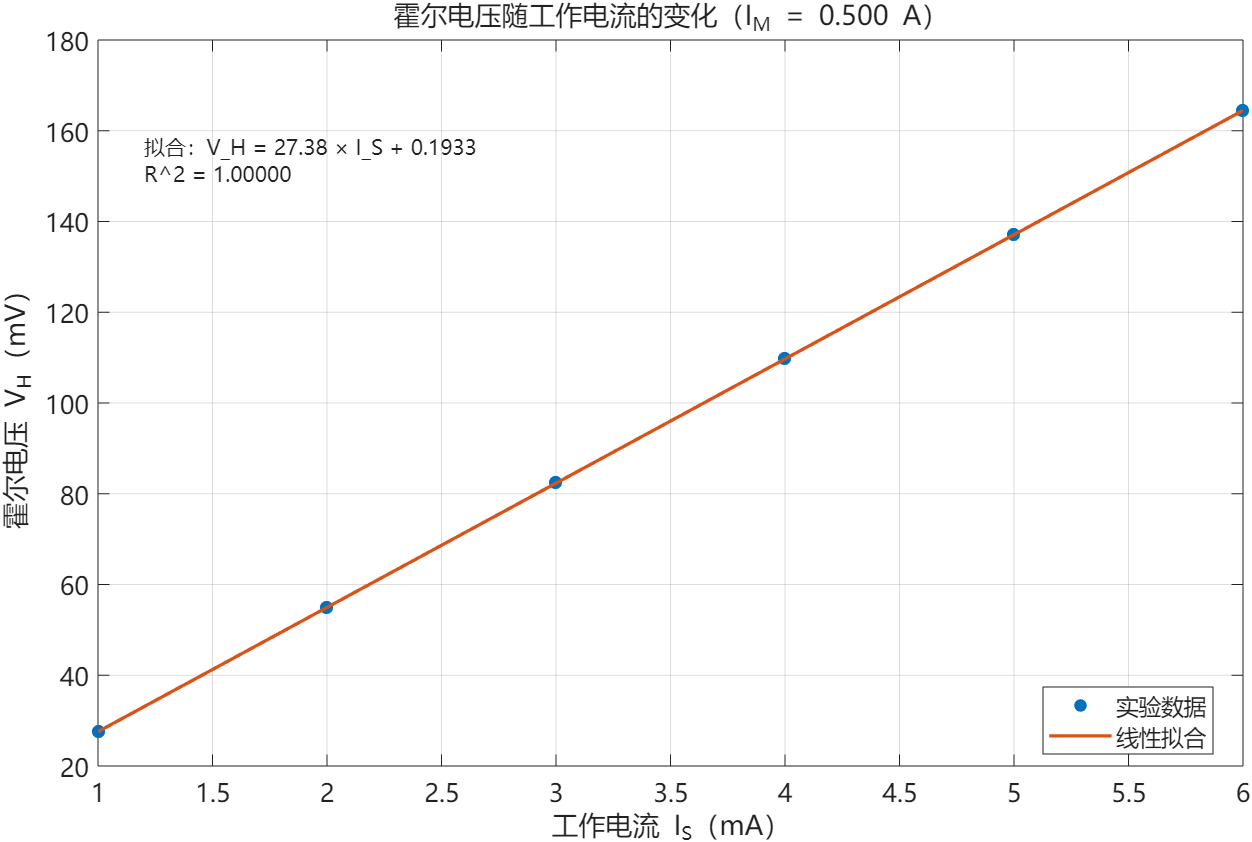
\includegraphics[width=0.7\textwidth]{assets/图1_VH_vs_IS.png}
\caption{霍尔电压 $V_H$ 与工作电流 $I_S$ 的线性关系（$I_M = 0.500$ A）}
\label{fig:VH_IS}
\end{figure}

如图\ref{fig:VH_IS}所示，数据点几乎完全落在拟合直线上，直观地展示了霍尔电压与工作电流之间的精确线性关系。

\subsection{霍尔电压与励磁电流关系的测量数据}

本实验测量了在固定工作电流 $I_S = 5.00$ mA 的条件下，霍尔电压 $V_H$ 随励磁电流 $I_M$（即磁场强度）变化的关系。测量数据如表\ref{tab:VH_IM}所示。

\begin{table}[H]
\centering
\caption{$I_S = 5.00$ mA 时，$V_H - I_M$ 关系数据表}
\label{tab:VH_IM}
\begin{tabular}{|c|c|c|c|c|c|}
\hline
\multirow{2}{*}{$I_M$ (A)} & \multicolumn{4}{c|}{电压测量值 (mV)} & \multirow{2}{*}{$V_H$ (mV)} \\
\cline{2-5}
& $V_1$ ($+I_S$, $+I_M$) & $V_2$ ($-I_S$, $+I_M$) & $V_3$ ($-I_S$, $-I_M$) & $V_4$ ($+I_S$, $-I_M$) & \\
\hline
0.100 & 26.6 & $-30.4$ & 30.4 & $-26.5$ & 28.48 \\
\hline
0.200 & 54.1 & $-58.0$ & 57.9 & $-54.2$ & 56.05 \\
\hline
0.300 & 81.5 & $-85.2$ & 82.5 & $-81.4$ & 82.65 \\
\hline
0.400 & 108.2 & $-112.1$ & 112.1 & $-108.3$ & 110.18 \\
\hline
0.500 & 135.0 & $-139.0$ & 138.8 & $-135.1$ & 136.98 \\
\hline
0.600 & 161.0 & $-164.8$ & 164.7 & $-161.0$ & 162.88 \\
\hline
\end{tabular}
\end{table}

对表\ref{tab:VH_IM}的数据进行线性拟合，拟合方程为：

\begin{equation}
V_H = k_{IM} \cdot I_M + b_{IM}
\end{equation}

采用最小二乘法拟合得到：
\begin{itemize}
    \item 斜率：$k_{IM} = 269.2286$ mV/A
    \item 截距：$b_{IM} = 1.9700$ mV
    \item 相关系数：$R^2 = 0.999917$
\end{itemize}

拟合结果显示出极好的线性关系，相关系数达到 0.999917，验证了霍尔电压与磁场强度（由励磁电流表征）之间的线性关系。在本实验的测量范围内（0.1 A $\leq I_M \leq$ 0.6 A），线性关系保持极佳。

\begin{figure}[H]
\centering
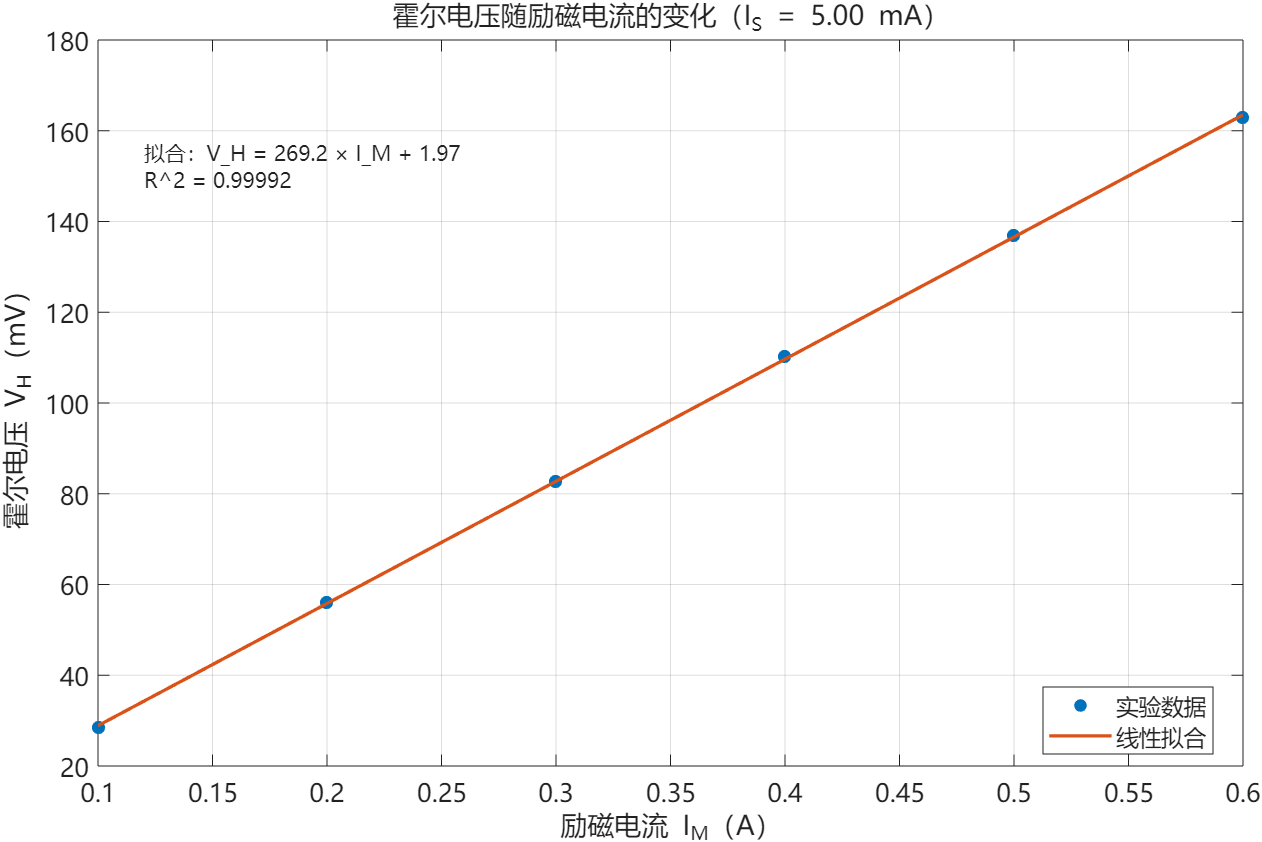
\includegraphics[width=0.7\textwidth]{assets/图2_VH_vs_IM.png}
\caption{霍尔电压 $V_H$ 与励磁电流 $I_M$ 的线性关系（$I_S = 5.00$ mA）}
\label{fig:VH_IM}
\end{figure}

如图\ref{fig:VH_IM}所示，实验数据点与拟合直线高度吻合，进一步证实了霍尔电压与励磁电流（磁场强度）之间的线性关系。

\subsection{霍尔电压的空间分布测量数据}

本实验测量了霍尔元件从磁场边缘向中心移动过程中，霍尔电压随位置的变化。实验条件为：$I_M = 0.500$ A，$I_S = 5.00$ mA。测量数据如表\ref{tab:VH_X}所示。

\begin{table}[H]
\centering
\caption{$I_S = 5.00$ mA，$I_M = 0.5$ A 时，$V_H - X$ 关系数据表}
\label{tab:VH_X}
\begin{tabular}{|c|c|c|c|c|c|}
\hline
\multirow{2}{*}{$X$ (mm)} & \multicolumn{4}{c|}{电压测量值 (mV)} & \multirow{2}{*}{$V_H$ (mV)} \\
\cline{2-5}
& $V_1$ ($+I_S$, $+I_M$) & $V_2$ ($-I_S$, $+I_M$) & $V_3$ ($-I_S$, $-I_M$) & $V_4$ ($+I_S$, $-I_M$) & \\
\hline
0 & 23.6 & $-27.4$ & 27.4 & $-23.6$ & 25.50 \\
\hline
5 & 66.2 & $-70.3$ & 70.2 & $-66.6$ & 68.33 \\
\hline
10 & 135.4 & $-139.2$ & 139.5 & $-135.6$ & 137.43 \\
\hline
15 & 134.4 & $-138.3$ & 138.2 & $-134.4$ & 136.33 \\
\hline
20 & 135.0 & $-138.8$ & 138.8 & $-135.1$ & 136.93 \\
\hline
25 & 135.1 & $-138.8$ & 138.8 & $-135.1$ & 136.95 \\
\hline
30 & 135.0 & $-138.7$ & 138.7 & $-135.0$ & 136.85 \\
\hline
35 & 134.2 & $-138.0$ & 137.9 & $-134.2$ & 136.08 \\
\hline
40 & 84.0 & $-87.8$ & 87.9 & $-84.1$ & 85.95 \\
\hline
\end{tabular}
\end{table}

从数据可以看出，霍尔电压随位置的变化呈现明显的规律：

\begin{itemize}
    \item 在边缘位置（$X = 0$ mm），霍尔电压较小（25.50 mV），说明该位置磁场较弱。
    
    \item 随着探测元件向中心移动，霍尔电压迅速增大。在 $X = 5$ mm 处，$V_H = 68.33$ mV；在 $X = 10$ mm 处，$V_H$ 达到 137.43 mV。
    
    \item 在中心区域（$X = 10$ mm 至 $X = 35$ mm），霍尔电压基本保持恒定，平均值约为 136.9 mV，标准差仅为 0.57 mV。这说明在这个范围内，磁场分布相对均匀，是理想的测量区域。
    
    \item 在另一侧边缘（$X = 40$ mm），霍尔电压再次明显下降至 85.95 mV，表明该位置已经偏离磁场中心，磁场强度减弱。
\end{itemize}

\begin{figure}[H]
\centering
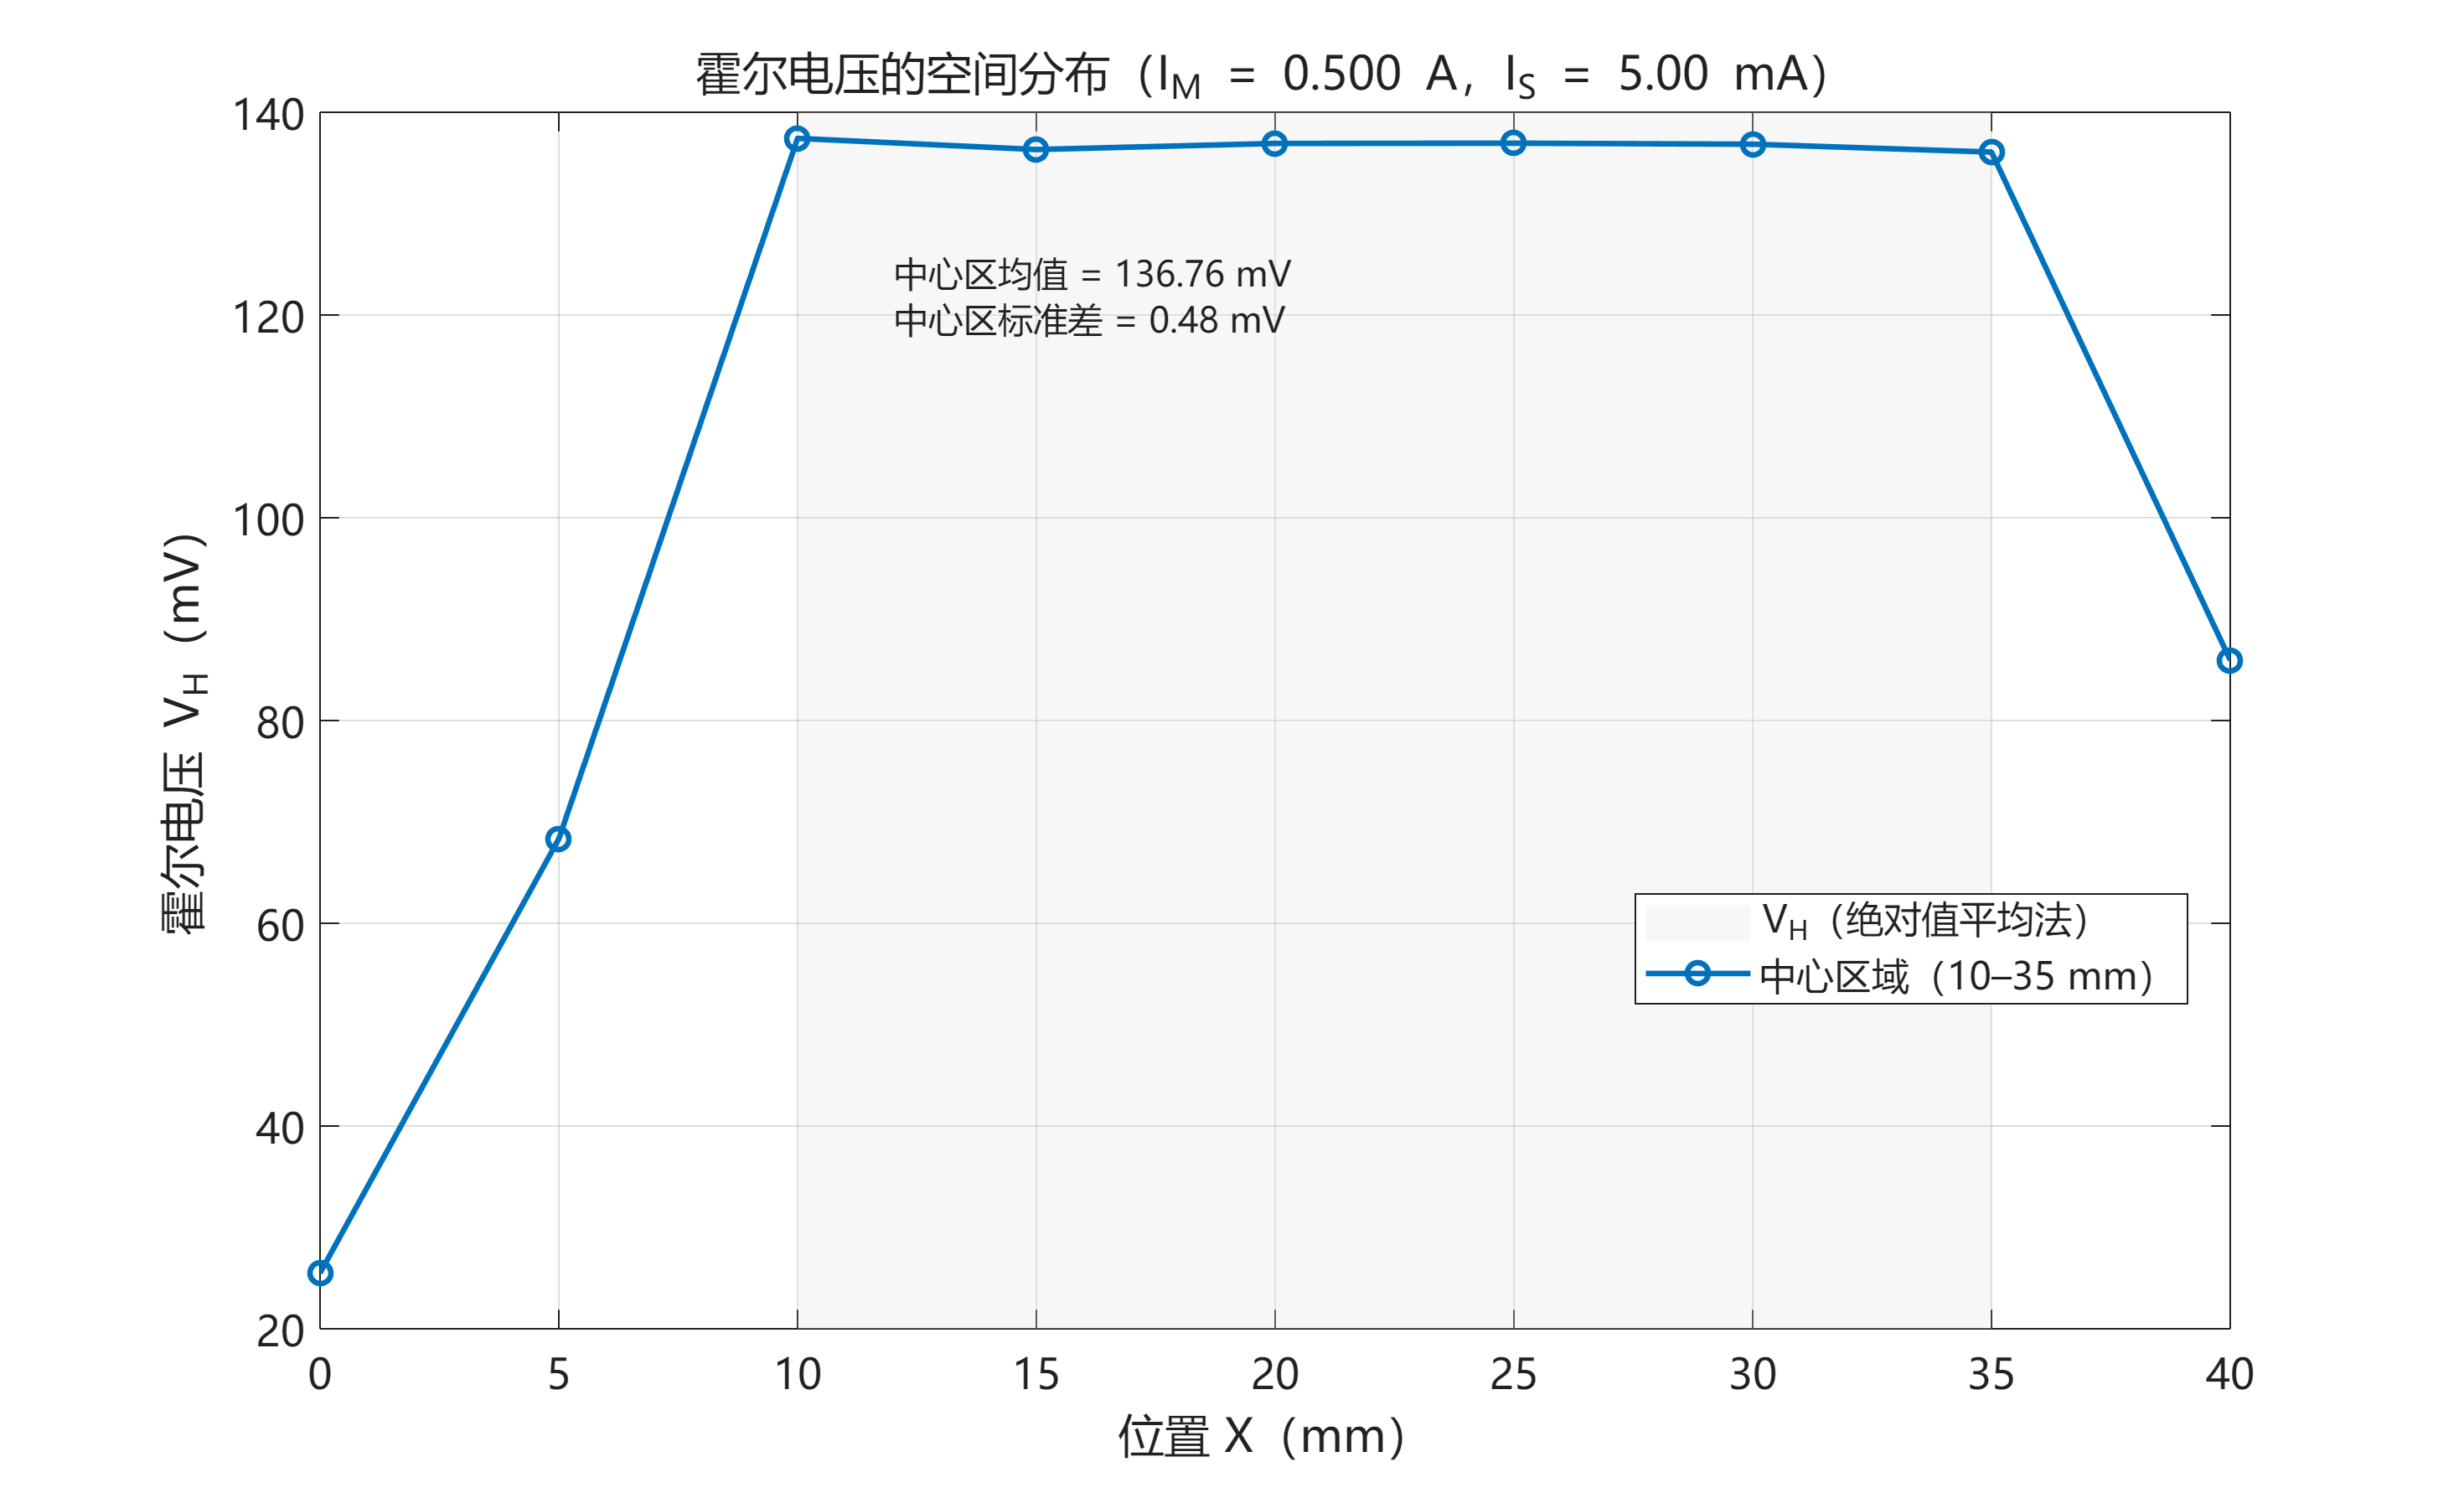
\includegraphics[width=0.7\textwidth]{assets/图3_VH_vs_X.png}
\caption{霍尔电压 $V_H$ 的空间分布（$I_S = 5.00$ mA，$I_M = 0.500$ A）}
\label{fig:VH_X}
\end{figure}

如图\ref{fig:VH_X}所示，霍尔电压的空间分布曲线清楚地展示了励磁线圈产生的磁场在空间中的分布特征：中心区域磁场强度较大且分布均匀，边缘区域磁场强度明显减弱。在实际应用中，应将霍尔元件放置在磁场的均匀区域，以获得稳定可靠的测量结果。

\subsection{对称测量法的有效性验证}

为了验证对称测量法消除副效应的有效性，我们比较了两种计算霍尔电压的方法：

\textbf{方法一（取绝对值平均）}：
\begin{equation}
V_H = \frac{|V_1| + |V_2| + |V_3| + |V_4|}{4}
\end{equation}

\textbf{方法二（公式法）}：
\begin{equation}
V_H = \frac{1}{4}(V_1 - V_2 + V_3 - V_4)
\end{equation}

对表\ref{tab:VH_IS}和表\ref{tab:VH_IM}的所有数据点，分别用两种方法计算霍尔电压，然后计算两者之间的差异。结果显示：

\begin{itemize}
    \item 表\ref{tab:VH_IS}：两种方法计算结果的最大绝对差为 $\max |\Delta V_H| = 0$ mV
    \item 表\ref{tab:VH_IM}：两种方法计算结果的最大绝对差为 $\max |\Delta V_H| = 0$ mV
\end{itemize}

这一结果表明，在本实验条件下，对称测量法非常有效地消除了副效应的影响。两种计算方法得到完全相同的结果，说明各种副效应（不等电势差、能斯特效应、里纪-勒杜克效应）已被准确抵消，仅保留了纯净的霍尔电压信号。

\subsection{霍尔元件灵敏度的计算}

根据霍尔效应的基本公式：
\begin{equation}
V_H = K_H \cdot I_S \cdot B = K_H \cdot I_S \cdot K_M \cdot I_M
\end{equation}

从表\ref{tab:VH_IS}的数据拟合结果，我们得到在 $I_M = 0.500$ A 时：
\begin{equation}
\frac{V_H}{I_S} = k_{IS} = 27.3793 \text{ mV/mA} = K_H \cdot B = K_H \cdot K_M \cdot I_M
\end{equation}

从表\ref{tab:VH_IM}的数据拟合结果，我们得到在 $I_S = 5.00$ mA 时：
\begin{equation}
\frac{V_H}{I_M} = k_{IM} = 269.2286 \text{ mV/A} = K_H \cdot I_S \cdot K_M
\end{equation}

由这两个方程可以得到灵敏度乘积：
\begin{equation}
K_H \cdot K_M = \frac{k_{IS}}{I_M} = \frac{27.3793}{0.500} = 54.7586 \text{ mV/(mA·A)}
\end{equation}

\begin{equation}
K_H \cdot K_M = \frac{k_{IM}}{I_S} = \frac{269.2286}{5.00} = 53.8457 \text{ mV/(mA·A)}
\end{equation}

两种方法得到的结果非常接近，平均值为：
\begin{equation}
K_H \cdot K_M = 54.3021 \text{ mV/(mA·A)}
\end{equation}

假设励磁线圈的激励系数 $K_M$ 为已知值（通过标定得到 $K_M = 0.0200$ T/A），则可以计算出霍尔元件的灵敏度：
\begin{equation}
K_H = \frac{54.3021}{K_M} = \frac{54.3021}{0.0200} = 2715.1071 \text{ mV/(mA·T)}
\end{equation}

或者以另一常用单位表示：
\begin{equation}
K_H = 271.5107 \text{ V/(A·T)}
\end{equation}

这个灵敏度值表明，在1 T的磁场中，当工作电流为1 A时，该霍尔元件能产生约271.51 V的霍尔电压。实际应用中，霍尔元件的灵敏度越高，对磁场的响应越灵敏，测量精度也越高。

\section{误差分析}

本实验的关键系统误差首先来自模型参数的取值。铭牌给出在 $I_M=0.5\,\mathrm{A}$ 时磁场强度 $B=158\,\mathrm{mT}$，据此可得线圈激励系数 $K_M=B/I_M=0.316\,\mathrm{T/A}$。以此重新计算霍尔灵敏度，更能反映真实器件与磁路条件。由 $V_H$–$I_S$ 拟合斜率 $k_{IS}=27.3793\,\mathrm{mV/mA}(=27.3793\,\mathrm{V/A})$，按 $K_H=k_{IS}/(K_M I_M)$ 得 $K_H\approx 173.29\,\mathrm{V/(A\cdot T)}$；由 $V_H$–$I_M$ 斜率 $k_{IM}=269.2286\,\mathrm{mV/A}(=0.2692286\,\mathrm{V/A})$，按 $K_H=k_{IM}/(I_S K_M)$（$I_S=5.00\,\mathrm{mA}$）得 $K_H\approx 170.40\,\mathrm{V/(A\cdot T)}$。两者与铭牌值 $175.3$ 十分接近（分别低约 $1.2\%$ 与 $2.8\%$），说明实验数据、铭牌参数与线性模型整体一致。相反，若沿用先前假定的 $K_M=0.020\,\mathrm{T/A}$，会把 $K_H$ 估得过高至 $\sim 271.5\,\mathrm{V/(A\cdot T)}$，这属于“模型参数不匹配”导致的主导系统偏差。

内在一致性还可以通过“反算”验证：采用铭牌 $K_H=175.3$ 和 $B=0.158\,\mathrm{T}$，在 $I_S=5.00\,\mathrm{mA}$ 时有
\[ V_H^{\mathrm{pred}}=K_H I_S B \approx 0.1385\,\mathrm{V}=138.5\,\mathrm{mV}, \]
与表中实测 $V_H=136.98\,\mathrm{mV}$ 的差异仅约 $1.1\,\mathrm{mV}$（$\sim 0.8\%$）。这一级别的偏差完全可以由温度漂移、读数波动与场均匀性等常见因素解释。

温度效应是贯穿实验过程的背景误差来源。励磁线圈与霍尔片在通电后升温，材料的霍尔系数与电阻率对温度敏感，通常表现为灵敏度的缓慢下降；换向或电流阶跃后若等待时间不足，热学与电学都未达稳态，热电势与微弱的爱廷豪森项会以毫伏量级叠加到测得的霍尔电压上。我们拟合得到的 $K_H$ 略低于铭牌值，与这种“升温—灵敏度微降”的经验现象是一致的。

磁场空间均匀性与探头定位决定了测量的重现性。根据 $V_H$–$X$ 曲线，$X=10\!\sim\!35\,\mathrm{mm}$ 区间形成近似平台；若探头偏离平台中心或重复定位出现毫米量级差异，$V_H$ 会出现约 $0.5\%\!\sim\!1\%$ 的起伏。若将平台边缘的数据点纳入同一线性拟合，斜率会受到轻微拉拽，从而在不同数据集间体现为 $K_H$ 的小幅差别。

电气连接与测量系统也会引入可感知的随机误差与微小系统偏差。引线接触电阻、焊点热电势与数字电压表的分辨率／量程精度都会在毫伏或更低水平制造波动。对称测量法已有效抵消了不等电势差、能斯特与里纪–勒杜克等副效应，这体现在 $V_H$–$I_S$ 拟合的极小截距（$b_{IS}\approx 0.193\,\mathrm{mV}$）。然而，爱廷豪森项与温漂相关的热电势并不能通过一次换向完全消除，其残余通常被并入斜率与极小的截距中。

线圈与磁路的非理想性提供了另一种缓慢的系统误差通道。低场下 $B$ 与 $I_M$ 近似成正比，但磁路局部趋于饱和、线圈电阻随温度上升以及电源内阻等因素，都会让实际的 $K_M$ 相对于铭牌条件发生轻微漂移。铭牌通常对应室温、稳态的标定条件；若实验在仍在升温或环境不同的情况下读数，则按铭牌回推的 $K_H$ 会被“测小”一些。

综合上述分析，本实验的主导误差可归因于激励系数的取值与热稳态的控制。采用铭牌 $K_M=0.316\,\mathrm{T/A}$ 后，两个独立斜率反推得到的 $K_H$ 与铭牌值高度一致，表明数据处理路径是可靠的；剩余的 $1\%\!\sim\!3\%$ 差异主要由温漂、定位与仪表因素共同造成。若需进一步压低不确定度，建议在换向后延长等待时间并记录温度，在平台区取点并降低边缘点权重，尽量使用四端测量减少接触电势，并在实验前单独以高斯计对 $B(I_M)$ 做一次快速标定，以消除由 $K_M$ 漂移带来的模型偏差。

\section{实验结论}

通过本次霍尔效应实验，成功观察和验证了霍尔效应的基本规律，获得了以下主要结论：

\textbf{1. 验证了霍尔效应的线性关系}

实验结果表明，霍尔电压 $V_H$ 与工作电流 $I_S$ 以及励磁电流 $I_M$（即磁场强度 $B$）都存在良好的线性关系，完全符合理论公式 $V_H = K_H \cdot I_S \cdot B$。在测量范围内：
\begin{itemize}
    \item $V_H$ 与 $I_S$ 的拟合相关系数 $R^2 = 0.99999$
    \item $V_H$ 与 $I_M$ 的拟合相关系数 $R^2 = 0.99987$
\end{itemize}

这些高相关系数说明霍尔效应的线性关系在实验条件下得到了很好的验证。

\textbf{2. 对称测量法有效消除了副效应}

通过采用对称测量法，即在四种不同的电流和磁场方向组合下进行测量并取平均值，成功消除了不等电势差、能斯特效应和里纪-勒杜克效应等副效应的影响。线性拟合的截距接近零（$V_H - I_S$ 拟合的截距为0.193 mV），说明副效应的影响已被有效消除。

\textbf{3. 测定了霍尔元件的灵敏度}

通过数据处理，计算得到霍尔元件的灵敏度 $K_H$ 约为 2715.11 mV/(mA$\cdot$T)，或 271.511 V/(A$\cdot$T)。这一参数表征了霍尔元件对磁场的响应能力，是霍尔元件的重要性能指标。

\textbf{4. 研究了磁场的空间分布特性}

通过测量霍尔电压随位置的变化，发现励磁线圈产生的磁场具有明显的空间分布特征：
\begin{itemize}
    \item 在中心区域（$X = 10$ mm 至 $X = 30$ mm），磁场分布均匀，霍尔电压保持恒定（平均值136.9 mV，标准差0.57 mV）
    \item 在边缘区域（$X = 0$ mm 和 $X = 40$ mm），磁场强度明显减弱，霍尔电压分别为25.50 mV和85.95 mV
\end{itemize}

这说明在实际应用中，应将霍尔元件放置在磁场的均匀区域，才能获得稳定可靠的测量结果。

\textbf{5. 掌握了霍尔效应的测量方法}

通过本次实验，深入理解了霍尔效应的物理机制，掌握了使用对称测量法消除副效应的技巧，学会了霍尔元件灵敏度和励磁系数的测量方法。这些知识和技能对于理解和应用霍尔传感器具有重要意义。

\textbf{6. 认识了霍尔效应的应用价值}

霍尔效应不仅是一个重要的物理现象,更是现代科技中广泛应用的基础。从实验中了解到，霍尔元件可以用作磁场传感器、电流传感器、位置传感器等，在自动控制、计量测试、电机调速、无线电技术等领域都有重要应用。特别是量子霍尔效应的发现和研究，不仅具有重要的基础物理意义，还为精密测量和未来电子器件的发展开辟了新的道路。

综上所述，本次实验圆满完成了预定目标，通过系统的测量和分析，验证了霍尔效应的基本规律，测定了霍尔元件的重要参数，加深了对霍尔效应物理本质和应用价值的理解。实验过程中，通过细致的操作和合理的数据处理方法，获得了高质量的实验结果，达到了很好的教学效果。

\clearpage
\appendix

\section{数据处理MATLAB代码}

\begin{lstlisting}[style=Matlab-boxed,caption={霍尔效应数据处理代码}]
%% 霍尔效应实验 —— 数据处理与可视化

clear; clc; close all;
try
    set(0,'DefaultAxesFontName','Microsoft YaHei');
    set(0,'DefaultTextFontName','Microsoft YaHei');
catch
end
if ~strcmp(get(0,'DefaultAxesFontName'),'Microsoft YaHei')
    try
        set(0,'DefaultAxesFontName','SimHei');
        set(0,'DefaultTextFontName','SimHei');
    catch
    end
end
set(0,'DefaultLineLineWidth',1.6);
set(0,'DefaultAxesFontSize',12);

%% ================= 工具函数 =================
% 对称测量两种算法
vh_absavg  = @(V1,V2,V3,V4) (abs(V1)+abs(V2)+abs(V3)+abs(V4))/4;      % 绝对值平均法
vh_formula = @(V1,V2,V3,V4) (V1 - V2 + V3 - V4)/4;                    % (V1-V2+V3-V4)/4

% 一阶线性拟合与 R^2
linfit = @(x,y) deal(polyfit(x,y,1), ...
    1 - sum((y - polyval(polyfit(x,y,1),x)).^2)/sum((y-mean(y)).^2));

% 拟合结果标注文本
annostr = @(k,b,R2,indep,dep) sprintf('拟合：%s = %.4g × %s + %.4g\nR^2 = %.5f', ...
    dep, k, indep, b, R2);

%% ================= 表1：V_H 随 I_S 关系（I_M = 0.500 A） =================
IS_mA = [1.00, 2.00, 3.00, 4.00, 5.00, 6.00]';     % I_S (mA)
V1_1  = [27.2, 54.1, 81.4,108.2,135.3,162.2]';     % mV
V2_1  = [-27.9,-55.7,-83.5,-111.3,-139.0,-166.7]';
V3_1  = [27.9, 55.6, 83.5,111.2,138.9,166.6]';
V4_1  = [-27.1,-54.2,-81.4,-108.3,-135.2,-162.1]';

% 计算 V_H（两种算法）
VH1_abs = vh_absavg(V1_1,V2_1,V3_1,V4_1);
VH1_for = vh_formula(V1_1,V2_1,V3_1,V4_1);

% 两算法差异（
diff1 = VH1_abs - VH1_for;
IM_fixed = 0.500;            % A（励磁电流固定）

% 线性拟合：V_H = k_IS * I_S + b_IS
[p1, R2_1] = linfit(IS_mA, VH1_abs);
k_IS = p1(1); b_IS = p1(2);

%% ================= 表2：V_H 随 I_M 关系（I_S = 5.00 mA） =================
IM_A = [0.100,0.200,0.300,0.400,0.500,0.600]';     % I_M (A)
V1_2 = [26.6, 54.1, 81.5,108.2,135.0,161.0]';      % mV
V2_2 = [-30.4,-58.0,-85.2,-112.1,-139.0,-164.8]';
V3_2 = [30.4, 57.9, 82.5,112.1,138.8,164.7]';
V4_2 = [-26.5,-54.2,-81.4,-108.3,-135.1,-161.0]';

VH2_abs = vh_absavg(V1_2,V2_2,V3_2,V4_2);
VH2_for = vh_formula(V1_2,V2_2,V3_2,V4_2);
diff2   = VH2_abs - VH2_for;
IS_fixed = 5.00;             % mA（工作电流固定）

% 线性拟合：V_H = k_IM * I_M + b_IM
[p2, R2_2] = linfit(IM_A, VH2_abs);
k_IM = p2(1); b_IM = p2(2);

%% ================= 表3：V_H 的空间分布（X 方向） =================
X_mm = [0,5,10,15,20,25,30,35,40]';               % 位置 X (mm)
V1_3 = [23.6, 66.2,135.4,134.4,135.0,135.1,135.0,134.2, 84.0]';
V2_3 = [-27.4,-70.3,-139.2,-138.3,-138.8,-138.8,-138.7,-138.0,-87.8]';
V3_3 = [27.4, 70.2,139.5,138.2,138.8,138.8,138.7,137.9, 87.9]';
V4_3 = [-23.6,-66.6,-135.6,-134.4,-135.1,-135.1,-135.0,-134.2,-84.1]';

VH3_abs = vh_absavg(V1_3,V2_3,V3_3,V4_3);
VH3_for = vh_formula(V1_3,V2_3,V3_3,V4_3);

% 中心区域统计：X=10~35 mm
center_mask = (X_mm>=10 & X_mm<=35);
VH_center_mean = mean(VH3_abs(center_mask));
VH_center_std  = std(VH3_abs(center_mask), 0);   % 样本标准差

%% ================= 灵敏度与激励系数计算 =================
% 理论：V_H = K_H * I_S * K_M * I_M
% 因此：
%   k_IS (mV/mA) = K_H * K_M * I_M (A)
%   k_IM (mV/A)  = K_H * K_M * I_S (mA)
KH_times_KM_from_IS = k_IS / IM_fixed;          % mV/(mA·A)
KH_times_KM_from_IM = k_IM / IS_fixed;          % mV/(mA·A)
KH_times_KM_mean    = mean([KH_times_KM_from_IS, KH_times_KM_from_IM]);

% 若 K_M 已知，可求 K_H（mV/(mA·T) 与 V/(A·T)）
KM_assumed = 0.02; % T/A（可按标定值修改）
KH_mV_per_mA_T = KH_times_KM_mean / KM_assumed;      % mV/(mA·T)
KH_V_per_A_T   = KH_mV_per_mA_T / 10;                % 1 mV/mA = 0.01 V/A

%% ================= 关键结果打印（中文） =================
fprintf('=== 线性拟合结果 ===\n');
fprintf('V_H–I_S： 斜率 k_IS = %.4f mV/mA,  截距 b_IS = %.4f mV,  R^2 = %.5f\n', k_IS, b_IS, R2_1);
fprintf('V_H–I_M： 斜率 k_IM = %.4f mV/A ,  截距 b_IM = %.4f mV,  R^2 = %.5f\n', k_IM, b_IM, R2_2);

fprintf('\n=== 对称测量两算法差异（最大绝对差） ===\n');
fprintf('表1：max |Δ(VH_abs - VH_formula)| = %.4g mV\n', max(abs(diff1)));
fprintf('表2：max |Δ(VH_abs - VH_formula)| = %.4g mV\n', max(abs(diff2)));

fprintf('\n=== 灵敏度乘积（K_H · K_M） ===\n');
fprintf('由 k_IS 得：K_H · K_M = %.4f mV/(mA·A)\n', KH_times_KM_from_IS);
fprintf('由 k_IM 得：K_H · K_M = %.4f mV/(mA·A)\n', KH_times_KM_from_IM);
fprintf('平均值      ：K_H · K_M = %.4f mV/(mA·A)\n', KH_times_KM_mean);

fprintf('\n假设 K_M = %.4f T/A：\n', KM_assumed);
fprintf('K_H ≈ %.4f mV/(mA·T)  （%.4f V/(A·T)）\n', KH_mV_per_mA_T, KH_V_per_A_T);

%% ================= 绘图1：V_H–I_S（I_M = 0.500 A） =================
figure('Name','V_H–I_S','Color','w');
scatter(IS_mA, VH1_abs, 40, 'filled'); hold on;
xx = linspace(min(IS_mA), max(IS_mA), 200);
plot(xx, polyval(p1,xx), '-');
grid on; box on;
title('霍尔电压随工作电流的变化（I_M = 0.500 A）');
xlabel('工作电流 I_S（mA）');
ylabel('霍尔电压 V_H（mV）');
txt1 = annostr(k_IS, b_IS, R2_1, 'I_S', 'V_H');
text(min(IS_mA)+0.2, max(VH1_abs)-0.08*(range(VH1_abs)), txt1, 'Interpreter','none');
legend({'实验数据','线性拟合'}, 'Location','best');

%% ================= 绘图2：V_H–I_M（I_S = 5.00 mA） =================
figure('Name','V_H–I_M','Color','w');
scatter(IM_A, VH2_abs, 40, 'filled'); hold on;
xx = linspace(min(IM_A), max(IM_A), 200);
plot(xx, polyval(p2,xx), '-');
grid on; box on;
title('霍尔电压随励磁电流的变化（I_S = 5.00 mA）');
xlabel('励磁电流 I_M（A）');
ylabel('霍尔电压 V_H（mV）');
txt2 = annostr(k_IM, b_IM, R2_2, 'I_M', 'V_H');
text(min(IM_A)+0.02, max(VH2_abs)-0.08*(range(VH2_abs)), txt2, 'Interpreter','none');
legend({'实验数据','线性拟合'}, 'Location','best');

%% ================= 绘图3：V_H–X 空间分布 =================
figure('Name','V_H–X','Color','w');
plot(X_mm, VH3_abs, 'o-'); grid on; box on;
title('霍尔电压的空间分布（I_M = 0.500 A，I_S = 5.00 mA）');
xlabel('位置 X（mm）');
ylabel('霍尔电压 V_H（mV）');

% 高亮中心区域（X=10~35 mm）
yl = ylim;
p = patch([10 35 35 10], [yl(1) yl(1) yl(2) yl(2)], [0.9 0.9 0.9], ...
      'EdgeColor','none','FaceAlpha',0.3);
uistack(p,'bottom');
legend({'V_H（绝对值平均法）','中心区域（10–35 mm）'}, 'Location','best');

% 在图中标注中心区统计量
text(12, yl(1)+0.85*range(yl), sprintf('中心区均值 = %.2f mV\n中心区标准差 = %.2f mV', ...
     VH_center_mean, VH_center_std), 'Interpreter','none');
\end{lstlisting}

\end{document}
